\documentclass{article}
\usepackage[T1]{fontenc}
\usepackage[utf8]{inputenc}
\usepackage{graphicx}
\usepackage{float}

\usepackage{hyperref}
\urlstyle{same}

\title{Wielowarstwowy system rekrutacji dla szkół z interfejsem webowym i aplikacją mobilną - technika TDD}
\author{Andrzej Westfalewicz, Filip Zyskowski}
\date{7 listopada 2019}

\renewcommand*\contentsname{Spis treści}
\renewcommand\refname{Odwołania} 

% do wrapowania tekstu w tabelce
\usepackage{array}
\newcolumntype{L}{>{\centering\arraybackslash}m{10cm}}
% 
\usepackage{tabularx}

\begin{document}

\begin{titlepage}
\maketitle
\end{titlepage}

\pagebreak

\section{Wstęp}

Technika TDD (Test-Driven Developement) jest techniką tworzenia oprogramowania, w której główną ideą jest w pierwszej kolejności pisanie testów do nieistniejącej funkcjonalności, a dopiero potem napisanie kodu implementującego tę funkcjonalność. Ten dokument będzie przedstawiał jak w naszym projekcie wygląda to podejście od strony implementacji kodu oraz uruchomienia środowiska testowego.

\section{Projekt testów}
Dzięki stworzonej już architekturze, w łatwy sposób możemy implementować kolejne funkcjonalności w technice TDD. Przejrzysta struktura i proste ich wywoływanie pozwala sprawnie i szybko przejść z pisania testów do samej implementacji.

\subsection{Struktura testów}
Projekt będzie testowany tylko pod względem logiki serwera. \\
Testy logiki znajdują się w folderze \emph{src/RecruitMe.Logic.Tests}. Struktura folderów odpowiada strukturze folderów projektu logiki (\emph{RecruitMe.Logic}), co znaczy tyle, że dla dowolnego pliku testu w projekcie testów, istnieje klasa testowana w tym samym folderze co plik testu, ale w projekcie logiki. \\

Testy zostały napisane z użyciem frameworka nUnit. Dla klas napisanych z pomocą tego narzędzia charakterystyczne są dwa atrybuty metod: \emph{Setup} - wskazująca metodę, która uruchamia się przed wykonaniem każdego testu, oraz \emph{Test} - oznaczającą pojedyńczy test. \\
W pojedyńczym pliku testu znajdzie się jedna metoda \emph{Setup} oraz co najmniej jedna metoda \emph{Test}.

\begin{figure}[H]
    \centering
    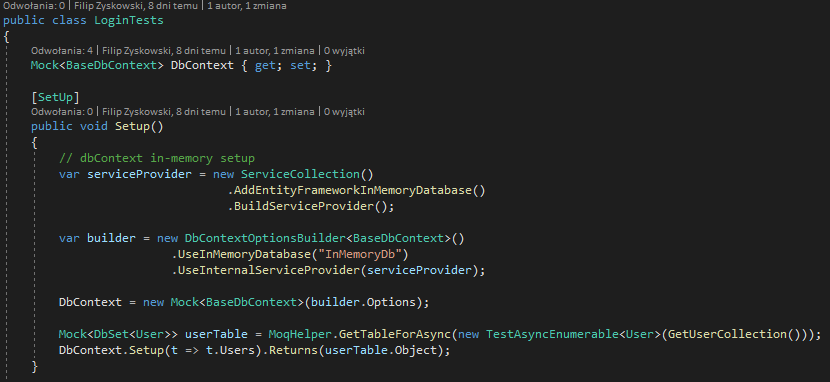
\includegraphics[width=1\linewidth]{images/setupTests.png}
    \caption{Metoda \emph{Setup()} uruchamiająca się przed każdym testem}
    \label{fig:test1_label}
\end{figure}

W metodzie \emph{Setup} będziemy zawsze tworzyć atrapę (\emph{mock}) bazy danych oraz używanej przez testowaną klasę tabeli/tabel. Tak stworzona atrapa pozwala w łatwy i powtarzalny sposób testować nasze metody, nie martwiąc się, że ewentualny błąd w metodzie zależy w jakiś sposób od bazy danych. \\

\begin{figure}[H]
    \centering
    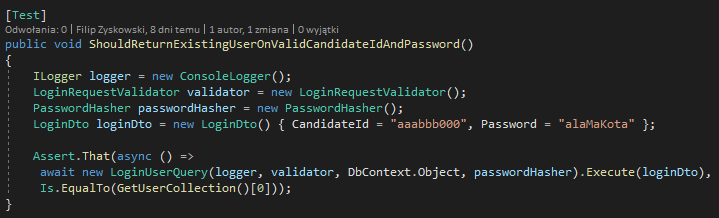
\includegraphics[width=1\linewidth]{images/testMethod.png}
    \caption{Przykładowy test}
    \label{fig:test2_label}
\end{figure}

W metodach oznaczonej atrybutem \emph{[Test]} znajduje się logika pojedyńczego testu. Wizualnie składa się z dwóch części: części przygotowania obiektów pod konkretny test oraz części działania i sprawdzenia w jednym. \\
Pierwsza część zawiera deklarację i inicjalizację obiektów potrzebnych do testu konkretnej funkcjonalności. Tutaj używane są klasy bez wewnętrznej logiki lub przetestowane już w innych testach. \\
Druga część posiada wywołanie funkcjonalności, którą chcemy przetestować. Wywołanie funkcjonalności jest częścią asynchronicznej metody anonimowej.
Sprawdzenie funkcjonalności sprowadza się do wyboru odpowiedniej metody z klasy \emph{Assert} i przekazania do niej wyżej wymienionej metody anonimowej.
Gdy chcemy sprawdzić, czy obiekt zwracany przez naszą testowaną funkcjonalność jest równy innemu, korzystamy wtedy z metody \emph{Assert.That}.

\subsection{Uruchomienie środowiska testowego}

Używając środowiska programistycznego \emph{Visual Studio} możemy łatwo sprawdzić czy napisane testy są napisane poprawnie oraz czy kod logiki jest zgodny z tymi testami.
Otwierając cały projekt w wyżej wymienionym programie, możemy kliknąć prawym klawiszem myszy na projekt testów (\emph{RecruitMe.Logic.Tests}) i kliknąć \emph{Run tests}. \\
Wyświetli się nam wtedy okienko z listą wszystkich dostępnych testów. Jednocześnie zostanie automatycznie uruchomione środowisko testowe, na którym będą przeprowadzane testy - będzie to widoczne po tym, że przy każdym teście w liście pojawi się kręcące się kółko. Sprawdzanie zakończy się, gdy przy każdym elemencie na liście pojawi się zielone lub czerwone kółko. Pojawienie się czerwonego kółka przy dowolnym z testów sprawia, że testy nie przechodzą poprawnie i wymagana jest interwencja w kodzie projektu - albo w samej logice testów, albo projektu.

Opcjonalnie, możemy również przeprowadzić testy uruchamiając w terminalu polecenie \emph{dotnet test RecruitMe.sln} (będąc w głównym folderze rozwiązania). Wymagane jest wtedy jednak przywrócenie i zbudowanie całego projektu odpowiednio poleceniami \emph{dotnet restore} oraz \emph{dotnet build}. Polecenia \emph{build} i \emph{test} uruchamiamy w konfiguracji \emph{Release}.

\begin{figure}[H]
    \centering
    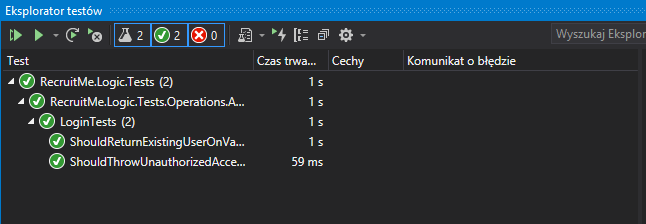
\includegraphics[width=1\linewidth]{images/runTest.png}
    \caption{Efekty uruchomienia testów}
    \label{fig:test3_label}
\end{figure}



\section{Historia dokumentu}

\begin{tabularx}{\linewidth}{|X|l|l|X|}
    \hline
    Autor & Data & Wersja & Wprowadzone zmiany \\
    \hline
    Filip Zyskowski & 06.12.2019 & v0.1 & Pierwsza wersja dokumentu \\
    \hline
\end{tabularx}

\end{document}
